% !TEX root = ./main.tex

\section{Quick-and-Dirty checks that can rule out good sampling}
\label{sec:quick}

\begin{wrapfigure}{r}{6cm}
  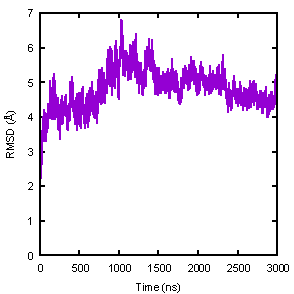
\includegraphics[width=5.8cm]{figures/rmsd/rmsd}
  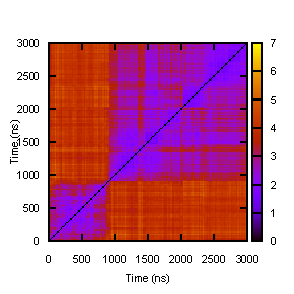
\includegraphics[width=5.8cm]{figures/rmsd/rmsds}
  \caption{
  \label{f:rmsd} RMSD as a measure of convergence.  The upper panel shows the
  $\alpha$-carbon RMSD of the protein rhodopsin from its starting structure as a
  function of time.  The lower panel shows the all-to-all RMSD map computed from the same
  trajectory.  Data from Leioatts, et al \cite{Grossfield-2015}.
  }
\end{wrapfigure}

It is difficult to establish with certainty that good sampling has been achieved, but it is not difficult to \emph{rule out} high-quality sampling.
Here we elaborate on some quick-and-dirty tests that quickly show inadequacies in sampling.

\subsection{Zeroth-order system-wide tests}

The simplest test for poor sampling is lack of equilibration: if the system is still noticeably relaxing from its starting conformation, statistical sampling has not even begun, and thus by definition is poor.  As a result, the very first test should be to verify that the basic equilibration has occurred.  To check for this, one should inspect the time series for a number of simple scalar values, such as potential energy, system size (and area, if you are simulating a membrane or other system where one dimension is distinct from the others), temperature (if you are simulating in the NVE ensemble), and/or density (if simulating in the isothermal-isobaric ensemble).  Often, simple visual inspection is sufficient to determine that the simulation is systematically changing, although more sophisticated methods have been proposed by Chodera \cite{Chodera-2016}.  If \emph{any} value appears to be systematically changing, then the system is not equilibrated.

\subsection{Tests based on configurational distance measures - e.g., RMSD for biomolecules}
We will use the standard biomolecular RMSD (root mean-squared difference) as a generic distance measure for illustrative purposes.
Alternatives to RMSD could be a dihedral-angle distance or another measure specific to your system of interest.
Note that RMSD, like any distance in a high-dimensional space, becomes ``degenerate'' for larger values: given a reference configuration, there are a large number of configurations which differ from the reference by a given large RMSD. This is analogous to the increasing number of points in three-dimensional space with increasing radial distance from a reference point, except much worse because of the dimensionality. For a detailed exploration of expected RMSD distributions for biomolecular systems see the work of Pitera.\citep{Pitera2014}

Some qualitative tools for assessing global sampling based on RMSD were reviewed
in prior work \cite{Grossfield2009}.   The classic time series plot of RMSD with
respect to a crystal or other single reference structure can immediately
indicate whether the structure is still systematically changing.  Although this
kind of plot was historically used as a sampling test, it should really be
considered as another equilibration test like those discussed above.  Moreover,
it's not even a particularly good test of equilibration, because the degeneracy
of RMSD means you can't tell if the simulation is exploring new states that are
equidistant from the chosen reference.  The upper panel of Figure \ref{f:rmsd}
shows a typical curve of this sort, taken from a simulation of the G
protein-coupled receptor rhodopsin \cite{Grossfield-2015}; the curve increases
rapidly over the few nanoseconds and then roughly plateaus.  It is difficult to
assign meaning to the other features on the curve.

A better RMSD-based convergence measure is the all-to-all RMSD plot; taking the
RMSD of each snapshot in the trajectory with respect to all others allows you to
use RMSD for what it does best, identifying very similar structures.  The lower
panel of Figure \ref{f:rmsd} shows an example of this kind of plot, applied to
the same trajectory before.  By definition, all such plots have values of zero
along the diagonal, and occupation of a given state shows up as a block of
similar RMSD along the diagonal; in this case, there are 2 main states, with one
transition occuring roughly 800 ns into the trajectory.  Off diagonal ``peaks''
(regions of low RMSD between structures sampled far apart in time) indicate that
the system is revisiting previously sampled states, a necessary condition for
good statistics.  In this case, the initial state is never sampled after the
first transition, but there are a number of small transitions within the second
state.

\subsection{Assessing Convergence}

\begin{wrapfigure}{r}{6cm}
  \includegraphics[width=5.8cm]{figures/combinedcluster/combinedcluster}
  \caption{
  \label{f:combinedcluster} Combined clustering between two independent trajectories as a measure of convergence. The X axis is the population of a cluster from trajectory 1, while the Y axis is the population of that cluster from trajectory 2. Cluster populations are show after 20, 100, and 800 ns of sampling. The simulations used to generate the data used in this plot are described in Roe et al.\citep{Roe2014}
  }
\end{wrapfigure}

Convergence in the context of biomolecular simulations typically refers to the overlap of two independent measurements of the same property. If a measure is not converged it is a strong indication that sampling is poor. There are two common ways to try to obtain independent measurements. Arguably the best way is to have multiple independent simulations, each with varying initial starting conditions. Ideally these starting conditions should in some way span the space to be sampled; this way one can have confidence that simulations are not being trapped in a local minimum. For example, say the goal is to sample the phi and psi torsions of alanine dipeptide: the phi and psi angles for one simulation could be started from an alpha-helical conformation, while another simulation could be started from a polyproline II conformation. It is important to note that the starting conditions only need to be varied enough so that the desired space is sampled. For example, if the goal is to sample protein folding and unfolding, there should be some simulations started from the folded conformation and some from the unfolded, but if it is not important to consider protein folding no initial conformation needs to be unfolded.

Another way to obtain independent measurements is to divide a single simulation into two or more subsets. However this can at times be problematic because it can be more difficult to tell if the system is trapped in a local minimum since there is a single starting point. Those employing this approach should take extra care to assess their results (see in particular sections on 'block averaging' below).

There are two simple ways to compare independent measurements of a property. The simplest is to compare the arithmetic means and standard deviations. If these values do not overlap then convergence has not been achieved. However, since this assumes that the values are normally distributed, a better way is compare the overlap of the probability distributions (i.e. the histograms). This can be done via Kullback-Leibler or Jensen-Shannon divergence.

\subsubsection{Combined Clustering}
One useful technique for evaluating convergence of structure populations is so-called "combined clustering". Briefly, in this method two or more independent trajectories are combined into a single trajectory, on which cluster analysis is performed. The resulting clusters are then split according to the trajectory they originally came from. If simulations are converged then each simulation will have the same population for any given cluster. Figure \ref{f:combinedcluster} shows results from combined clustering of two independent trajectories as a plot of cluster population fraction from the first trajectory compared to the second. If the two independent trajectories are perfectly converged then all points should fall on the X=Y line. As simulation time increases the cluster populations from the independent trajectories are in better agreement, which indicates the simulation is converging. For another example of performing combined cluster analysis see Bergonzo et al.